% %%%%%%%%%%%%%%%%%%%%%%%%%%%%%%%%%%%%%%%%%%%%%%%%%%%%%%
% This file contains the text for the common 
% introductory chapter.
% %%%%%%%%%%%%%%%%%%%%%%%%%%%%%%%%%%%%%%%%%%%%%%%%%%%%%%

\section{Introduction}%
\label{sec:introduction}

This here is a dummy text for testing text editions. Whoever reads this text is
own fault. The text only indicates the grey value of the font. Is it really like that? Is it
whether I write: ``This is a blind text'' or ``Huardest gefburn''? Kjift mitnichten! A dummy text provides me with important information. I use it to measure the readability 
of a typeface, its impression, how harmonious the figures are in relation to each other
and check how wide or narrow it is. A dummy text should contain as many different 
letters as possible and be set in the original language. It does not have to
It does not have to make sense, but it should be readable. Foreign-language texts such as ``Lorem ipsum'' do not serve the purpose 
the actual purpose, as they give a false impression.


Figure~\ref{fig:mri} shows an example of MR images. There is much literature on the normalisation
of intensities in MR images (e.\,g.~\cite{Jaeger09}). 


\begin{figure}[h]
\centering
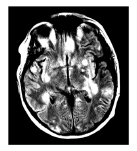
\includegraphics[height=4cm]{Figures/jaeger1.png}
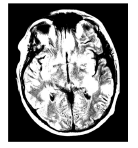
\includegraphics[height=4cm]{Figures/jaeger2.png}
\caption{An example of MR images (taken from \cite{Jaeger09}).}%
\label{fig:mri}
\end{figure}
